\chapter{Energy Reconstruction}
\label{sec:energy}
	The~second stage is the~reconstruction of the~particle's energy using a~fit of its reconstructed track (see Section~\ref{sec:track}). We have tested three ways of reconstructing the~energy. Fitting is done using the~MINUIT algorithm implemented in ROOT~\cite{ROOT}. \textcolor{red}{Cite some CERN article directly on MINUIT, can add a~section.}
	
	The~\textbf{Cubic Spline Fit} is a~tested and later rejected method of energy reconstruction. It uses smoothly connected piecewise cubic polynomials between uniformly spaced nodes. Energy is calculated using the~fit parameters by computing the~radius of curvature in different points of the~fitted curve using the~known magnitude of the~magnetic field perpendicular to the~trajectory. We rejected this method because tuning of the~fit to have a~reasonably stable radius of curvature turned out to be unpractical.
	
	The~\textbf{Circle and Lines Fit} was chosen as an~alternative since this corresponds to the~shape of a~trajectory of a~charged particle crossing a~finite volume with a~homogeneous magnetic field. The~energy of the~particle can be estimated using the~fitted radius and the~magnitude of the~perpendicular magnetic field in the~middle of the~\ac{TPC}.
	
	The~\textbf{Runge-Kutta Fit} uses the~4th order Runge-Kutta numerical integration described in Section~\ref{sec:rks}. Initial parameters of the~track (including the~particle's energy) are optimized so that the~integrated trajectory fits to the~reconstructed one. This fit can also be performed as a~single parameter (i.e., energy) fit if we get the~initial position and orientation of the~particle on the~entrance to the~\ac{TPC} from previous detectors (\ac{Tpx3} and \ac{MWPC}, see Section~\ref{sec:IEAP}).
	
	\begin{figure}
		\centering
		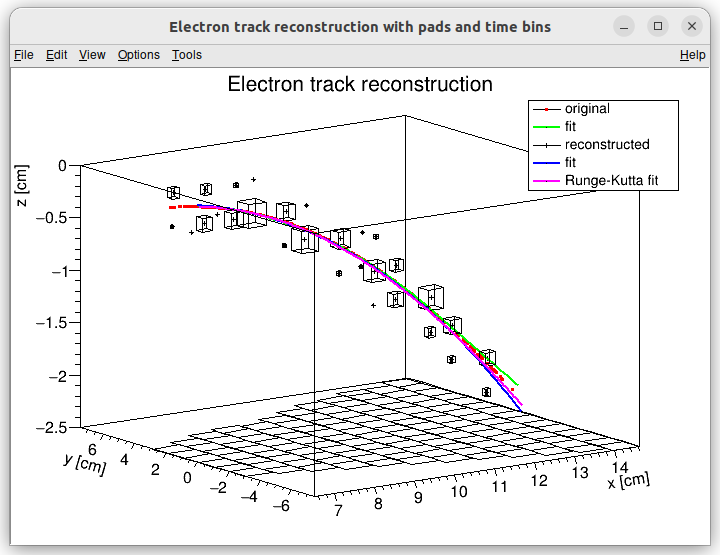
\includegraphics[width=0.5\textwidth]{9010_3d.png}
		\caption{Example of a~fitted reconstructed track. \textcolor{red}{Swap for better image.}}
		\label{fig:90103d}
	\end{figure}
	
	\section{Cubic Spline Fit}
	\label{sec:cspline}
		The~first attempt to get an~early estimate of the~kinetic energy of the~particle uses a~cubic spline fit. We use an~electron track starting in the~origin of our coordinate system with an~initial direction in the~positive $x$~axis. The~ example track is simulated microscopically (see Section~\ref{sec:microsim}) with a~kinetic energy of 8~MeV in a~gas mixture 90\%~Ar~+~10\%~CO$_2$ (the~same track was used in Section~\ref{sec:trackfirst}). \textcolor{red}{This track should probably be described in the~simulation chapter.}
				
		In order to calculate the~spline, we use the~class \textit{TSpline3} from ROOT. This allows us to evaluate the~spline using the~coordinates $(x_n,z_n)$ of each node and the~derivatives $d_1,d_2$ in the~first and the~last node. We can fit these parameters of a~fixed amount of nodes to the~simulated trajectory. We use the~IMPROVE algorithm provided by the~\textit{TMinuit} class in ROOT. This algorithm attempts to find a~better local minimum after converging.
		
		After the~fit, we want to get an~energy estimate. In order to calculate it, we need the~radius of curvature, which we get from the~fitted spline at every point of the~trajectory. The~part of the~spline corresponding to a~given node is defined as
			\begin{equation}
				z(x) = z_n + b \Delta x+c(\Delta x)^2+d(\Delta x)^3,
			\end{equation}
		where $\Delta x = x-x_n$ and $b,c,d$ are coefficients. Using this equation, we derive the~radius of curvature\footnote{For the~general formula see \url{https://en.wikipedia.org/wiki/Curvature\#Graph_of_a_function}} as:
			\begin{equation}
				r(x) = \frac{\left(1+z'^2(x)\right)^\frac{3}{2}}{z''(x)} = \frac{\left(1+\left(b+2c\Delta x+3d(\Delta x)^2\right)^2\right)^\frac{3}{2}}{2c+6d\Delta x}.
			\end{equation}
		Based on the~geometry of the~detector, we can assume the~magnetic field \linebreak$\bm{B}(x,0,z) = (0,B(x,z),0)$ for a~track in the~XZ~plane. Since the~electron is relativistic, the~effect of the~electric field on its trajectory is negligible. The~Lorentz force $F_L$ is then always perpendicular to the~momentum of the~electron and acts as a~centripetal force $F_c$:
			\begin{linenomath}
			\begin{align}
				\bm{F_L} &= \bm{F_c},\\
				\norm{e\bm{v}\times\bm{B}} &= \frac{\gamma m_e v^2}{r},\\
				e c\beta B &= \frac{E_{0e} \beta^2}{r\sqrt{1-\beta^2}},\\
				\sqrt{1-\beta^2} &= \frac{E_{0e} \beta}{ecBr},
			\end{align}
			\end{linenomath}
			\begin{equation}
				\beta^2(x) = \left[1+\left(\frac{E_{0e}}{ecB(x,z(x))r(x)}\right)^2\right]^{-1}, \label{eq:ekin1}
			\end{equation}
		where $e$~is the~elementary charge, $c$~is the~speed of light in vacuum, $m_e$~is the~rest mass of electron, $E_{0e} = m_e c^2$ is the~corresponding energy, $\gamma$~is the~Lorentz factor, $\bm{v}$~is the~velocity of the~electron, and $\beta = \frac{v}{c}$. We can then finally get our estimate of the~kinetic energy for a~given point on the~trajectory as follows:
			\begin{equation}
				\label{eq:ekin2}
				E_\text{kin}(x) = \left(\frac{1}{\sqrt{1-\beta^2(x)}}-1\right)E_{0e}.
			\end{equation}
		We can then average these estimates at multiple points to get one final estimate. This method was later rejected in favor of the~circle and lines fit described in Section~\ref{sec:clines}.
		\textcolor{red}{Add some figures.}
		
		\begin{figure}
			\centering
			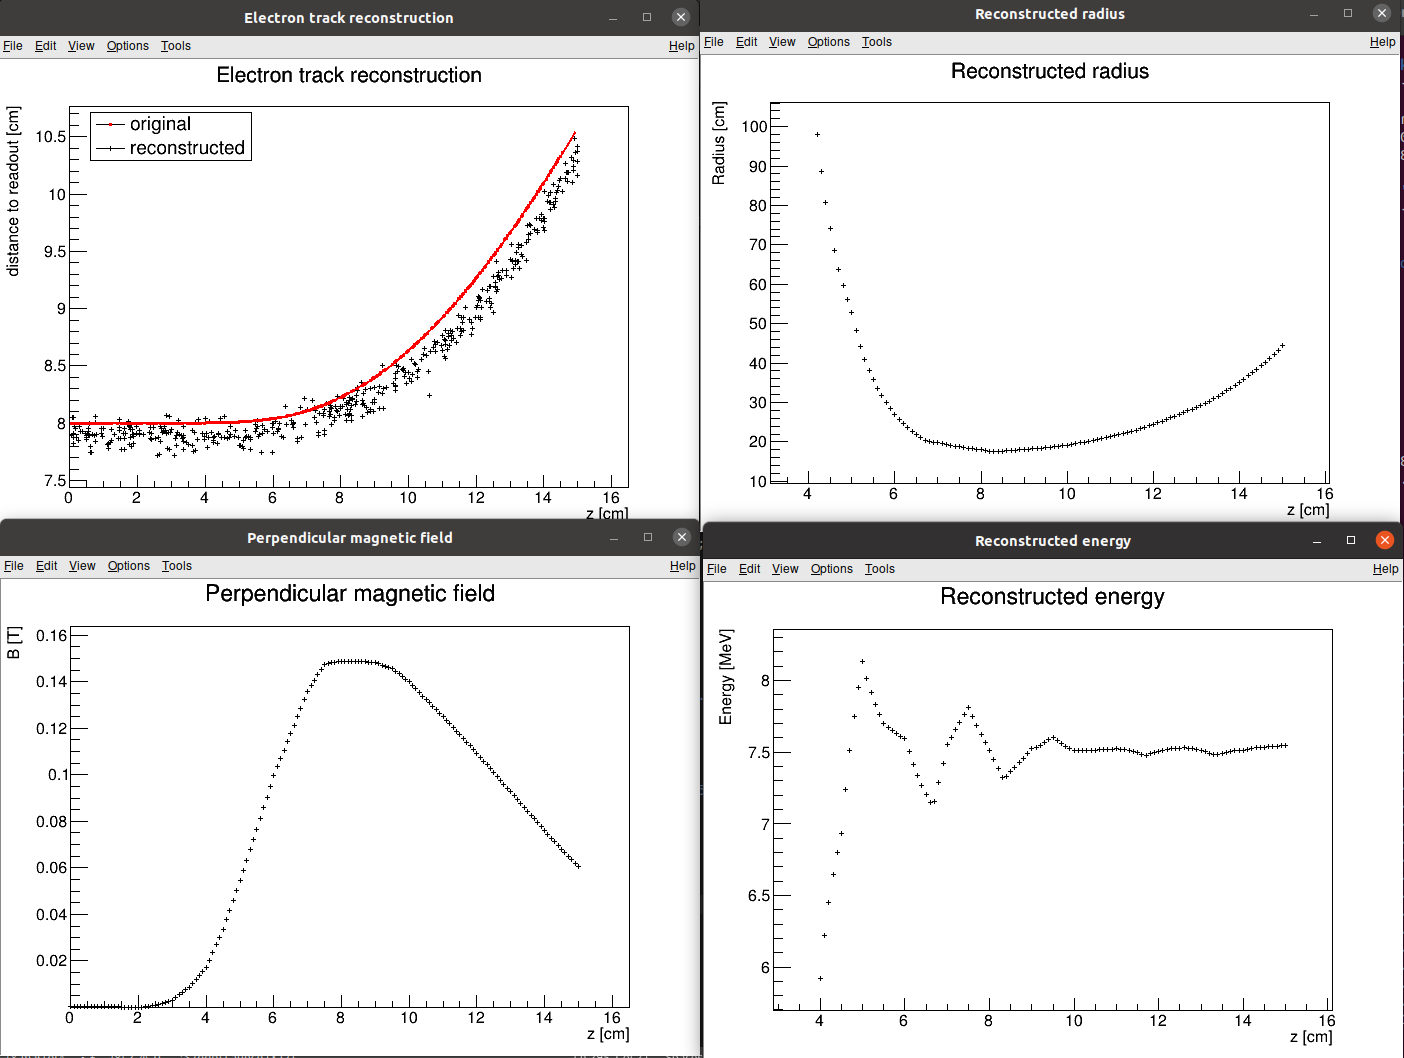
\includegraphics[width=0.8\textwidth]{9010_splines.png}
			\caption{First attempt at a~track reconstruction using only the~drift velocity. Spline energy reconstruction attempt. \textcolor{red}{Swap for better image(s) -- subfigure environment, correct coordinates.}}
			\label{fig:9010splines}
		\end{figure}
	
	\section{Circle and Lines Fit}
	\label{sec:clines}
		Another way to estimate the~particle's kinetic energy is to~fit its trajectory with a~circular arc with lines attached smoothly. This shape of trajectory corresponds to a~movement of a~charged particle through a~homogeneous magnetic field perpendicular to the~particle's momentum and limited to a~certain volume. In general, the~shape of such a~trajectory in a~non-perpendicularly oriented field is a~spiral. In our case, this component is negligible since the~field is approximately toroidal and the~particle motion is nearly perpendicular to it. At first, we tested a~2D version of this fit, then we adapted it to 3D.
		
		Our field is not homogeneous, it is therefore not entirely clear what value of magnetic field should be used along with the~fitted radius (using equations~\ref{eq:ekin1} and~\ref{eq:ekin2}) to get the~best estimate for the~kinetic energy. Since we only use this method as the~first iteration of the~particle's energy that we later refine, an~optimal solution of this problem is not required. Instead, we tested two options: taking the~value of the~field in the~middle of the~fitted circular arc and taking the~average field along it. \textcolor{red}{We haven't really tried to plot this for multiple tracks, but these estimates are saved somewhere and could be plotted.}
		
		\subsection{Two-dimensional fit}
			In the~2D case, the~fitted function used for the~electron track\footnote{Electron tracks bend towards negative~$z$, we need to use the~upper part of the~circle} described in Section~\ref{sec:cspline} is defined as follows: \textcolor{red}{Maybe describe this track that we used at the~beginning somewhere earlier (section microscopic simulations \textrightarrow~Testing track?) so that it is easier to refer to it in multiple sections. It is not part of the~early GitHub commits, so maybe it won't be possible to create exact replicas of the~images, but they should be at least very similar.}
				\begin{equation}
					\label{eq:clines2d}
					z(x) = \begin{cases}
								a_1x+b_1 & x<x_1\\
								z_0+\sqrt{r^2-(x-x_0)^2} & x_1\leq x\leq x_2\\
								a_2x+b_2 & x>x_2
						   \end{cases},
				\end{equation}
			where $a_{1,2}$ and $b_{1,2}$ are the~parameters of the~lines, $(x_0,z_0)$ is the~center of the~circle, $r$ is its radius, and $(x_{1,2},z_{1,2})$ are the~coordinates of the~function's nodes. That means we have 9~parameters ($z_{1,2}$ are not used in the~function) along with 2~continuity conditions and 2~smoothness conditions. For the~fit, we use the~coordinates of the~nodes and the~radius of the~circle, which gives us 5~independent parameters (only the~radius has to be larger than half of the~distance between nodes). The~continuity conditions (combined with the~relations for $z_{1,2}$) are as follows:
				\begin{equation}
					\label{eq:ccont}
					z_{1,2} = a_{1,2}x_{1,2}+b_{1,2} = z_0-\sqrt{r^2-(x_{1,2}-x_0)^2}.
				\end{equation}
			The~smoothness conditions are as follows:
				\begin{equation}
					\label{eq:a12}
					a_{1,2} = \frac{x_0-x_{1,2}}{\sqrt{r^2-(x_{1,2}-x_0)^2}}.
				\end{equation}
			Equation~\ref{eq:ccont} gives us the~values of $b_{1,2}$
				\begin{equation}
					\label{eq:b12}
					b_{1,2} = z_{1,2} - a_{1,2} x_{1,2}.
				\end{equation}
			For the~coordinates of the~center of the~circle, we can use the~fact that the~center has to lie on the~axis of its chord. In other words, there is a~value of a~parameter~$t$ such that, using the~parametric equation of the~axis
				\begin{equation}
					\begin{pmatrix} x_0\\ z_0 \end{pmatrix} = \begin{pmatrix} \frac{x_1+x_2}{2}\\ \frac{z_1+z_2}{2} \end{pmatrix} + t \begin{pmatrix} \frac{z_2-z_1}{2}\\ \frac{x_1-x_2}{2} \end{pmatrix}.
				\end{equation}
			At the~same time, the~center has to be in a~distance of $r$ from the~nodes:
				\begin{linenomath}
				\begin{gather}
					(x_1-x_0)^2 + (z_1-z_0)^2 = r^2,\\
					\left(\frac{x_1-x_2}{2}+\frac{z_1-z_2}{2}t\right)^2 + \left(\frac{z_1-z_2}{2}+\frac{x_2-x_1}{2}t\right)^2 = r^2,\\
					\left(\left(\frac{x_2-x_1}{2}\right)^2+\left(\frac{z_2-z_1}{2}\right)^2\right)t^2+\left(\frac{x_2-x_1}{2}\right)^2+\left(\frac{z_2-z_1}{2}\right)^2-r^2=0.
				\end{gather}
				\end{linenomath}
			Since our electron track bends towards negative $z$ and $x_2 > x_1$, we only care about the~solution with $t>0$
				\begin{equation}
					t = \sqrt{\frac{r^2}{\left(\frac{x_2-x_1}{2}\right)^2+\left(\frac{z_2-z_1}{2}\right)^2}-1},
				\end{equation}
				\begin{align}
					x_0 = \frac{x_1+x_2}{2} + \frac{z_2-z_1}{2} \sqrt{\frac{r^2}{\left(\frac{x_2-x_1}{2}\right)^2+\left(\frac{z_2-z_1}{2}\right)^2}-1},\label{eq:x0}\\
					z_0 = \frac{z_1+z_2}{2} - \frac{x_2-x_1}{2} \sqrt{\frac{r^2}{\left(\frac{x_2-x_1}{2}\right)^2+\left(\frac{z_2-z_1}{2}\right)^2}-1}.\label{eq:z0}
				\end{align}
			The~function defined in Equation~\ref{eq:clines2d} along with equations~\ref{eq:a12}, \ref{eq:b12}, \ref{eq:x0} and~\ref{eq:z0} derived using the~continuity and smoothness conditions (combined with the~relations for $z_{1,2}$) fully define our fitted function with parameters $r,x_{1,2},z_{1,2}$. \textcolor{red}{Some pictures of the~fit on the~tested track. Results of the~fit. Again, the~actual fit uses 8-z. Use GeoGebra schematics to generate a~picture of 2D geometry.}
			
			\textcolor{red}{Tested on a~Runge-Kutta sample, and with microscopic tracks + map simulation. Preliminary 2D version (done) and complete 3D version. Geometry of the~fit with its derivation.}
			
			\begin{figure}
				\centering
				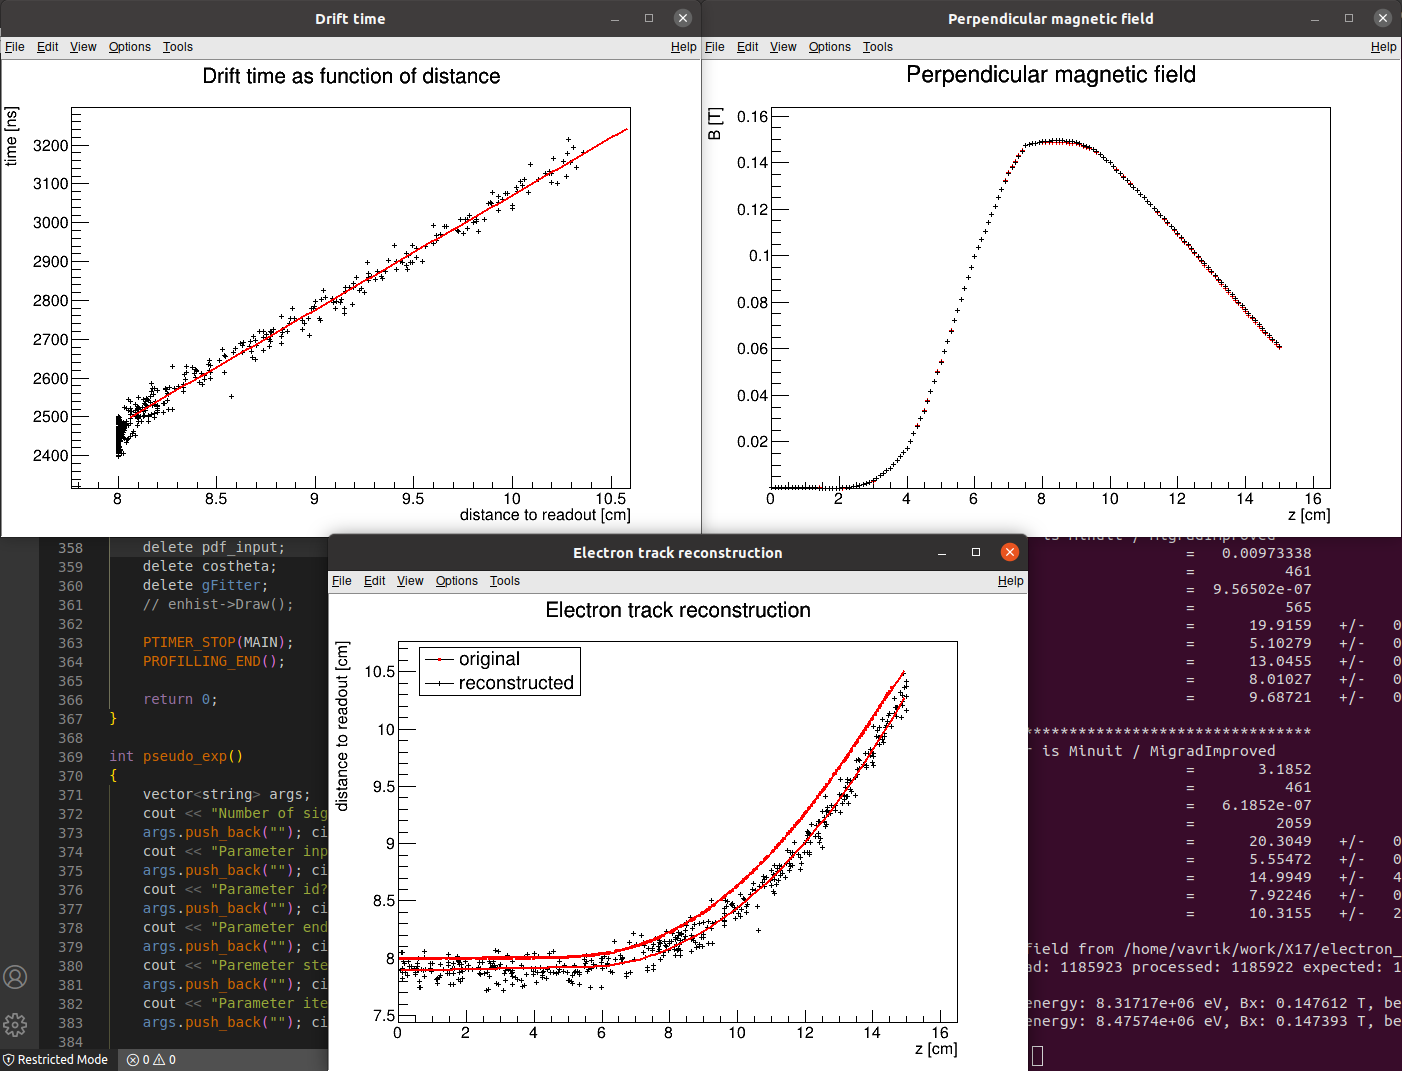
\includegraphics[width=0.8\textwidth]{9010_circle2D.png}
				\caption{First attempt at a~track reconstruction using only the~drift velocity. Circle and Lines Fit in 2D. \textcolor{red}{Swap for better image, correct coordinates.}}
				\label{fig:9010circle2D}
			\end{figure}
		
		\subsection{Three-dimensional fit}
			\textcolor{red}{Explain the geometry and least square method used for the~3D fit.}
			
			\begin{figure}
				\centering
				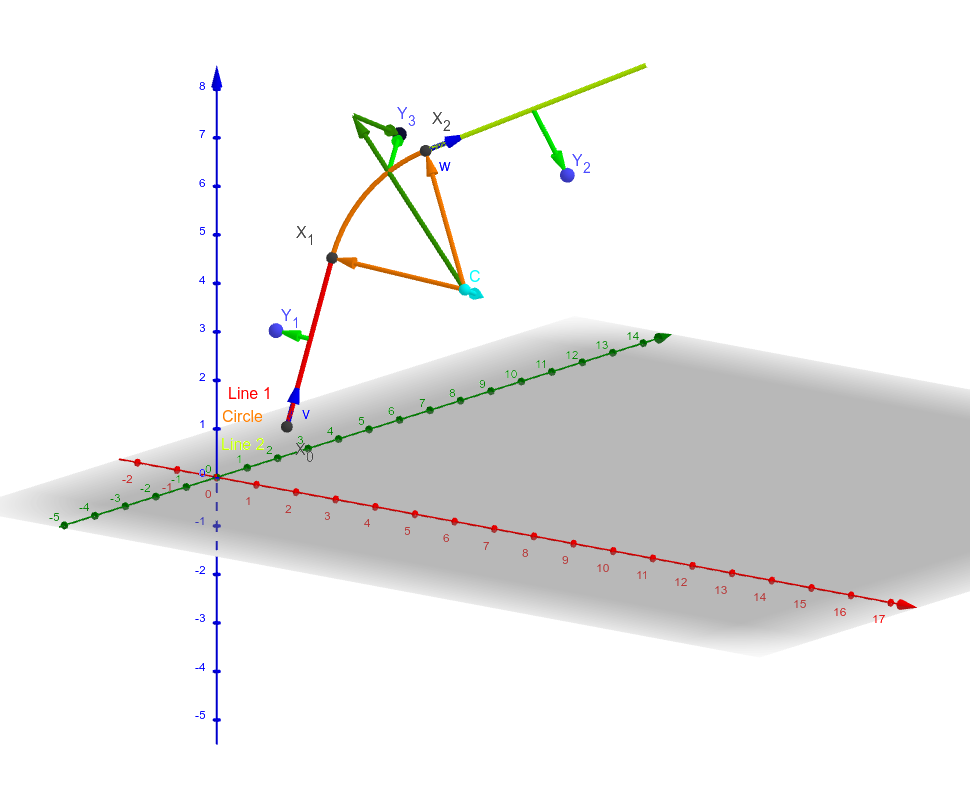
\includegraphics[width=0.8\textwidth]{circlefit.png}
				\caption{Circle and Lines Fit 3D geometry. \textcolor{red}{Swap for better image.}}
				\label{fig:circlefit}
			\end{figure}
	
	\section{Runge-Kutta Fit}
		\textcolor{red}{Single parameter fit with 4th order Runge-Kutta simulated track. Future testing with microscopic simulations and map simulation. Derivation of the~geometry (least squares).}